\documentclass[12pt]{article}
\setlength{\oddsidemargin}{0in}
\setlength{\evensidemargin}{0in}
\setlength{\textwidth}{6.5in}
\setlength{\parindent}{0in}
\setlength{\parskip}{\baselineskip}

\usepackage{amsmath,amsfonts,amssymb}
\usepackage{graphicx}
\usepackage{fancyhdr}
\usepackage[]{algorithmicx}
\usepackage{tikz-qtree}
\pagestyle{fancy}

\usepackage{graphicx}
\graphicspath{ {./images/} }

\begin{document}

\lhead{{\bf CSCI 3104: Algorithms \\ Problem Set 4} }
\rhead{{\bf Oscar Delfado \\ Summer 2019, CU-Boulder}}
\renewcommand{\headrulewidth}{0.4pt}

% 15+45+20+20=100 points possible

\vspace{-3mm}
\begin{enumerate}

	% -- MEDIUM PROBLEM
	\item \textit{ (15 points) Shadow is writing a secret message to Harry and wants to prevent it from being understood by Thormund. He decides to use Huffman encoding to encode the message. Magically, the symbol frequencies of the message are given by the Lucas numbers, a famous sequence of integers discovered by the same person who discovered the Fibonacci numbers. The nth Lucas number is defined as $L_n = L_{n-1} + L_{n-2}$ for $n > 1$ with base cases $L_0$ = 2 and $L_1$ = 1.}
	\begin{enumerate}
	\item\textit{  \label{q:huff:a} For an alphabet of $\Sigma=\{a,b,c,d,e,f,g,h\}$ with frequencies given by the first $|\Sigma|$ Lucas numbers, give an optimal Huffman code and the corresponding encoding tree for Shadow to use.}
	
a=2, b=1, c=3, d=4, e=7, f=11, g=18, h=29, 



\begin{tikzpicture}[level distance=1.5cm,
  level 1/.style={sibling distance=3cm},
  level 2/.style={sibling distance=1.5cm}]
  \node {75}
    child {node {$h=29^0$}}
      child {node {$46^1$}
		child {node{$g=18^0$}}
		  child {node{$28^1$}
			 child {node{$f=11^0$}}
				child{node{$17^1$}
					child {node{$e=7^0$}}
						child{node{$10^1$}
							child {node{$d=4^0$}}
								child{node{$6^1$}
									child {node{$c=3^0$}}
									child{node{$3^1$}
										child {node{$b=1^0$}}
										child{node{$a=2^1$}}
							}
						}
					}
				}
			}
		};
\end{tikzpicture}


\begin{table}[]
\begin{tabular}{ll}
(This is for part a but for some reason wouldn't compile correctly) \\
  a & 1111111 \\
  b & 1111110 \\
  c & 111110 \\
  d & 11110 \\
  e & 1110 \\
  f & 110 \\
  g & 10 \\
  h & 0 \\ 
\end{tabular}
\end{table} 

	\end{enumerate}

\item\textit{  Generalize your answer to (\ref{q:huff:a}) and give the structure of an optimal code when the frequencies are the first $n$ Lucas numbers.}
	


\begin{table}[]
\begin{tabular}{lll}
  Optimal Code \\
  a & 11,...,11 (n-1)  \\
  b & 11,..11 (n-2) + 0 \\
  c & 11,...,11(n-3) + 0 \\
  . & . \\
  . & . \\
  . & . \\
  z & 0
\end{tabular}
\end{table}
	
This works because everytime we we up the Lucas number it will never make a seperate tree that would added to the original. This is because when we want to add the n Lucas number, the the n+1 Lucas number would be greater than $\Sigma{L_{n-1}}$ so the n Lucas number and and the root would make children of the new root with their frequencies added. Therefor the tree left childrens will all be letters and there for going up the tree it would be the amount of "1" decreases while ending with zero with the expection of a.

\newpage

	% HARD PROBLEM
	\item \textit{ (45 points) A good hash function $h(x)$ behaves in practice very close to the uniform hashing assumption analyzed in class, but is a deterministic function. That is, $h(x)=k$ each time $x$ is used as an argument to $h()$. Designing good hash functions is hard, and a bad hash function can cause a hash table to quickly exit the sparse loading regime by overloading some buckets and under loading others. Good hash functions often rely on beautiful and complicated insights from number theory, and have deep connections to pseudorandom number generators and cryptographic functions. In practice, most hash functions are moderate to poor approximations of uniform hashing.}
	
	\smallskip \textit{ Consider the following hash function. Let $U$ be the universe of strings composed of the characters from the alphabet $\Sigma=[${\tt A}$,\dots,${\tt Z}$]$, and let the function $f(x_{i})$ return the index of a letter $x_{i}\in \Sigma$, e.g., $f(${\tt A}$)=1$ and $f(${\tt Z}$)=26$. Finally, for an $m$-character string $x\in \Sigma^{m}$, define $h(x) = \left(\left[\sum_{i=1}^{m}f(x_{i})\right]\!\! \mod \ell\right)$, where $\ell$ is the number of buckets in the hash table. That is, our hash function sums up the index values of the characters of a string $x$ and maps that value onto one of the $\ell$ buckets.}
	
	\begin{enumerate}
    	\item\textit{  The following list contains US Census derived last names: }\\
    	\textit{ {\tt http://www2.census.gov/topics/genealogy/1990surnames/dist.all.last} }\\
    	\textit{ Using these names as input strings, first choose a uniformly random 50\% of these name strings and then hash them using $h(x)$.}
    	
    \textit{ 	Produce a histogram showing the corresponding distribution of hash locations when $\ell=200$. Label the axes of your figure. Briefly describe what the figure shows about $h(x)$, and justify your results in terms of the behavior of $h(x)$. Do not forget to append your code.}
    	 
    	{\footnotesize Hint: the raw file includes information other than name strings, which will need to be removed; and, think about how you can count hash locations without building or using a real hash table.}

 \begin{figure}
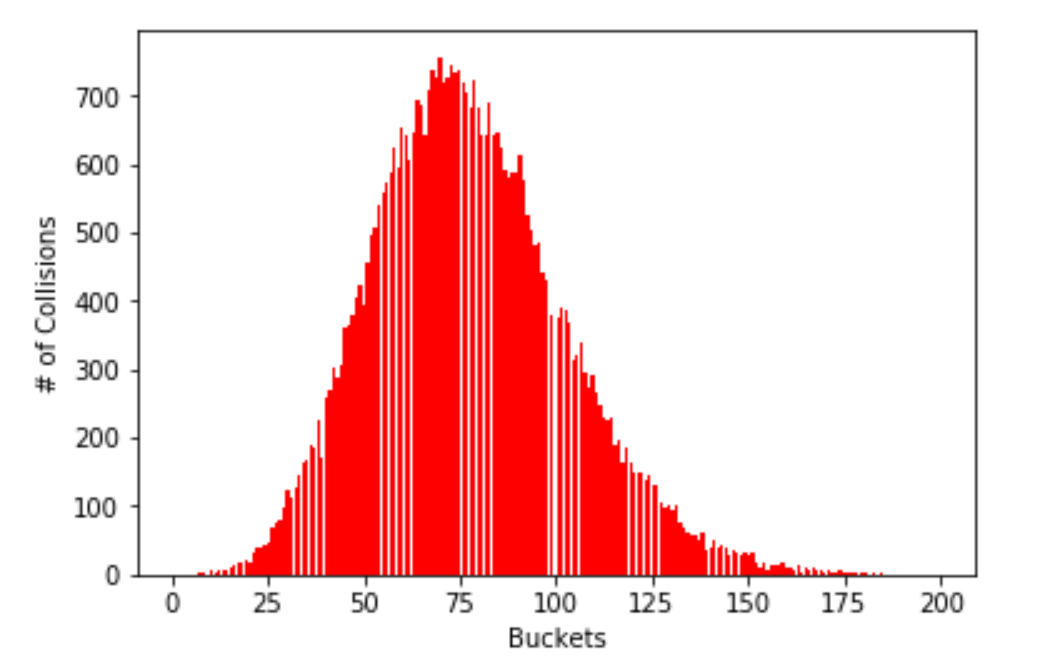
\includegraphics[scale=.5 ]{Graph}
	There is a lot of collisions in the 50-90 range of the buckets, overloading them pretty severely.
\end{figure}

\newpage
    	\item \textit{ Enumerate at least 4 reasons why $h(x)$ is a bad hash function relative to the ideal behavior of uniform hashing.}

	1. The distribution of is not nearly spread evenly enough to be a good uniform hashing function.\\
	2. h(x) does not account for the letters positions in each name.\\
	3. Last names have a general limit to how long they are going to be, and because h(x) is partly based off of the length of a name, the hash locations are limited toa certain possible number. This number is not nearly as large as the amount of names, and thus is a bad way to create hash locations.\\

    	
    	\item\textit{  Produce a plot showing (i) the length of the longest chain (were we to use chaining for resolving collisions under $h(x)$) as a function of the number $n$ of these strings that we hash into a table with $\ell=200$ buckets, (ii) the exact upper bound on the depth of a red-black tree with $n$ items stored, and (iii) the length of the longest chain were we to use a uniform hash instead of $h(x)$. Include a guide of $c\,n$}
    	
    	\textit{ Then, comment (i) on how much shorter the longest chain would be under a uniform hash than under $h(x)$, and (ii) on the value of $n$ at which the red-black tree becomes a more efficient data structure than $h(x)$ and separately a uniform hash.}
	\end{enumerate}
	
\newpage

	% MEDIUM PROBLEM
	\item \textit{ (20 points) Grog is struggling with the problem of making change for $n$ cents using the smallest number of coins for his purchase of a new great sword. Grog has coin values of $v_{1}<v_{2}<\dots<v_{r}$ for $r$ coin types, where each coin's value $v_{i}$ is a positive integer. His goal is to obtain a set of counts $\{d_{i}\}$, one for each coin type, such that $\sum_{i=1}^{r}d_{i}=k$ and where $k$ is minimized.}
	\begin{enumerate}
	\item \textit{ A greedy algorithm for making change is the \textbf{cashier's algorithm}, which all young wizards learn. Harry writes the following pseudocode on the whiteboard to illustrate it, where $n$ is the amount of money to make change for and $v$ is a vector of the coin denominations:}
	%
	\begin{small}
	\begin{verbatim}
	wizardChange(n,v,r) :
	   d[1 .. r] = 0       // initial histogram of coin types in solution
	   while n > 0 {
	      k = 1
	      while ( k < r and v[k] > n ) { k++ }
	      if k==r { return 'no solution' }
	      else { n = n - v[k] }
	   }
	   return d
	\end{verbatim}
	\end{small}
	\textit{ Thormund snorts and says Harry's code has bugs. Identify the bugs and explain why each would cause the algorithm to fail.}

	Bugs: \\
	1. On line 2 is should be d[0...r-1] as the indexing seems to start at 0.
	2. On line 4 (k=1) should be k=r-1 because it should start with the largest coins first and should also be before the first while loop as it won't restart with the largest coin in the beginning of 1st loop. \\
	3. On line 5 (k<r) is unessasary and messes up the loop so it is better removed and (v[k]>n) should be v[k]<=n like this once the coin is unable to fit it will move on to the next smalles coin. \\
	4. On line 6 (k==r) should be k==-1 as this means its gone through all the coins and still couldn't hit the desire amount (n). \\
	5. On line 7 the else is unessary as the if statements returns and also it needs to add all number of coins used in d[k] so we can add d[k]++ if this wasn't there it would do the work but return 0's.\\
	6  lastly k++ should not be done inside the second loop and should be done on the end of the first while loop so the same can can be subtracteds from n as much as it could. earlier it would only do it once then move on to the next and so not subtracting correctly.\\
	
	\item\textit{  Sometimes the dwarves at Rocky Mountain Bank run out of coins,}%
	%
	\footnote{It's a little known secret, but dwarven pets like to \textit{eat} the coins. It isn't pretty for the coins, in the end.}
	%
	\textit{ and make change using whatever is left on hand. Identify a set of U.S. coin denominations for which the greedy algorithm does not yield an optimal solution. Justify your answer in terms of optimal substructure and the greedy-choice property. (The set should include a penny so that there is a solution for every value of $n$.)}

One subset of Euro USA denominations in which the greedy algorithm fails to provide the optimal solution is the subset v = (1, 10, 25) for the n = 34 cents. Firstly it would get the largest coin 25 and one to it, when it does this the remaingin is 9 so it skips coin(10) and goes to coin(1) which he adds 9 making a total of 10 coins used $<9,0,1>$. The optimal solution would be $<4,3,0> (1(4)+10(3) = 34$) as you can see the best solution only used 7 coins compare to 10 that greedy used. Firstly it doesn' have Optiumal Substructure as $30 \leq n \leq 33$ which are subsolution to 34 are not optimal("Best" Solutions) with the greedy choice property as when we choose n=30 the greedy choice would give $<5, 0, 1>= 6$ when optimal $<0,3,0>=3$, so the greedy choice property fails to pick best solution.

	
%	1. Greedy-choice property: A global optimum can be arrived at by selecting a local optimum.
%	2. Optimal substructure: An optimal solution to the problem contains an optimal solution to subproblems.
	
	\item \textit{ On the advice of wizards specializing in electricity, Rocky Mountain Bank has announced that they will be changing all  coin denominations into a new set of coins denominated in powers of $c$, i.e., denominations of $c^{0}, c^{1}, \dots , c^{\ell}$ for some integers $c>1$ and $\ell\geq 1$.  (This will be done by a spell that will magically transmute old coins into new coins, before your very eyes.) Prove that the cashier's algorithm will always yield an optimal solution in this case.}
	
	\textit{ Hint: first consider the special case of $c=2$.}

(Answer)

	\end{enumerate}
    
\newpage

    \item\textit{  (20 points) We saw in the previous problem that the cashier's (greedy) algorithm for making change doesn't handle arbitrary denominations optimally. In this problem you'll develop a dynamic programming solution which does, but with a slight twist. Suppose we have at our disposal an arbitrary number of \emph{cursed} coins of each denomination $d_1, d_2, \dotsc, d_k$, with $d_1 < d_2 < \dotsc < d_k$, and we need to provide $n$ cents in change. We will always have $d_1=1$, so that we are assured we can make change for any value of $n$. The curse on the coins is that in any one exchange between people, with the exception of $i=2$, if coins of denomination $d_i$ are used, then coins of denomination $d_{i-1}$ \emph{cannot} be used. Our goal is to make change using the minimal number of these cursed coins (in a single exchange, i.e., the curse applies).}

    \begin{enumerate}
    	\item\textit{  For $i \in \{1,\dotsc,k\}$, $n \in \mathbb{N}$, and $b \in \{0,1\}$, let $C(i,n,b)$ denote the number of cursed coins needed to make $n$ cents in change using only the first $i$ denominations $d_1, d_2, \dotsc, d_i$, where $d_{i-1}$ is allowed to be used if and only if $i \leq 2$ or $b=0$. That is, $b$ is a Boolean ``flag'' variable indicating whether we are excluding denomination $d_{i-1}$ or not ($b=1$ means exclude it). 	}
    	Write down a recurrence relation for $C$ and prove it is correct. Be sure to include the base case.
    	\item \textit{ Based on your recurrence relation, describe the order in which a dynamic programming table for $C(i,n,b)$ should be filled in.}
    	
    	\item\textit{  Based on your description in part (b), write down pseudocode for a dynamic programming solution to this problem, and give a $\Theta$ bound on its running time (remember, this requires proving both an upper \emph{and} a lower bound).}
    \end{enumerate}

\end{enumerate}

\end{document}


